\documentclass[CJK,final,t]{beamer}
\mode<presentation>
{
%  \usetheme{Warsaw}
%  \usetheme{Aachen}
%  \usetheme{Oldi6}
%  \usetheme{I6td}
%  \usetheme{I6dv}
  \usetheme{thu}
%  \usetheme{I6pd}
%  \usetheme{I6pd2}
%	\usetheme{Berlin}
}
% additional settings
\usepackage[orientation=landscape,size=custom,width=200,height=120,scale=1.9]{beamerposter}
\listfiles
\graphicspath{{figures/}}

%\setbeamerfont{itemize}{size=\normalsize}
%\setbeamerfont{itemize/enumerate body}{size=\normalsize}
%\setbeamerfont{itemize/enumerate subbody}{size=\normalsize}

% additional packages
%\usepackage{times}
\usepackage{pgf,tikz}
\usepackage{amsmath,amsthm, amssymb, latexsym}
\usefonttheme[onlymath]{serif}
\boldmath

\usepackage[BoldFont,SlantFont,CJKchecksingle,xeCJKactive]{xeCJK}
\setCJKmainfont[BoldFont=SimHei]{SimSun}
\setCJKmonofont{SimSun}% 设置缺省中文字体

%\usepackage{utf8}
%\usepackage[utf8]{inputenc}
%\usepackage{inputenc}                % load it without argument to avoid Babel warnings
%\usepackage[vietnam,USenglish]{babel} % T5 font encoding


%\usepackage{exscale}
%\boldmath
\usepackage{booktabs, array}
%\usepackage{rotating} %sideways environment
%\usepackage[]{babel}
%\usepackage[utf8]{inputenc}
% Display a grid to help align images
%\beamertemplategridbackground[1cm]
%\newtheorem{problem}{问题}
\newtheorem{asm}{假定}
%\newtheorem{theorem}{定理}
%\newtheorem{theorem}{Theorem}
%\newtheorem{definition}{定义}
%\newtheorem{definition}{Definition.}
%\newtheorem{lemma}{引理}
%\newtheorem{corollary}{推论}
%\newtheorem{corollary}{Corollary}
%\newtheorem{proposition}{命题}
%\newtheorem{example}{例}
%\newtheorem{remark}{注}
%\newtheorem{solution}{解答}
\newcommand\term[1]{#1}
\def\semichecked{\checkmark\!\!\!\raisebox{0.4 em}{\tiny$\smallsetminus$}}
\definecolor{Gray}{gray}{0.75}
\newcommand{\argmax}{\operatornamewithlimits{argmax}}
\newcommand{\argmin}{\operatornamewithlimits{argmin}}

\title{\huge 事件日志完备性分析与噪声处理研究}
\author[杨和东等]{杨和东, 闻立杰, 王建民}
\institute[THSS]{清华大学软件学院,中国北京}
\date[\date]{\today}

% abbreviations
\usepackage{xspace}
\makeatletter
\DeclareRobustCommand\onedot{\futurelet\@let@token\@onedot}
\def\@onedot{\ifx\@let@token.\else.\null\fi\xspace}
\def\eg{{e.g}\onedot} \def\Eg{{E.g}\onedot}
\def\ie{{i.e}\onedot} \def\Ie{{I.e}\onedot}
\def\cf{{c.f}\onedot} \def\Cf{{C.f}\onedot}
\def\etc{{etc}\onedot}
\def\vs{{vs}\onedot}
\def\wrt{w.r.t\onedot}
\def\dof{d.o.f\onedot}
\def\etal{{et al}\onedot}
\makeatother

%%%%%%%%%%%%%%%%%%%%%%%%%%%%%%%%%%%%%%%%%%%%%%%%%%%%%%%%%%%%%%%%%%%%%%%%%%%%%%%%%%%%%%%%%%%%%%%%%%%%%%%%%%%%
%%%%%%%%%%%%%%%%%%%%%%%%%%%%%%%%%%%%%%%%%%%%%%%%%%%%%%%%%%%%%%%%%%%%%%%%%%%%%%%%%%%%%%%%%%%%%%%%%%%%%%%%%%%%
\begin{document}
\begin{frame}{} 
  \begin{columns}[t]
    \begin{column}{.3\linewidth}

      %%%%%%%%%%%%%%%%%%%%%%%%%%%%%%%%%%%%%%%%%%%%%%%%%%%%%%%%%%%%%%%%%%%%%%%%%%%%%%%%%%%%%%%%%%%%%%%%%%%%%%%%%%%%

      \begin{block}{问题、挑战与思路}
\indent{过程挖掘是业务过程管理的一个重要研究领域,过程挖掘技术可以从记录业务过程运行历史情况的事件日志中抽取各种有价值的信息,为业务过程的改进提供支撑。过程发现是过程挖掘的重点研究内容,旨在从事件日志中挖掘出业务过程的模型,但\alert{日志的完备性}(包括全局信息完备性与局部信息完备性)问题与\alert{噪声问题}迟迟没有得到满意的解决,严重地影响了过程挖掘的进一步发展及其在现实生活中的应用。}

\indent{完备性要求日志包含过程模型的全部特定信息(比如行为信
息),噪声导致日志中的有些轨迹跟过程模型的实际运行情况不符,完备性与噪声
都是相对于产生日志的过程模型而言的。在过程发现问题中,产生日志的过程模
型是未知的,这是这两个问题的共同难点所在。}
		  
\noindent{%
	\begin{center}
	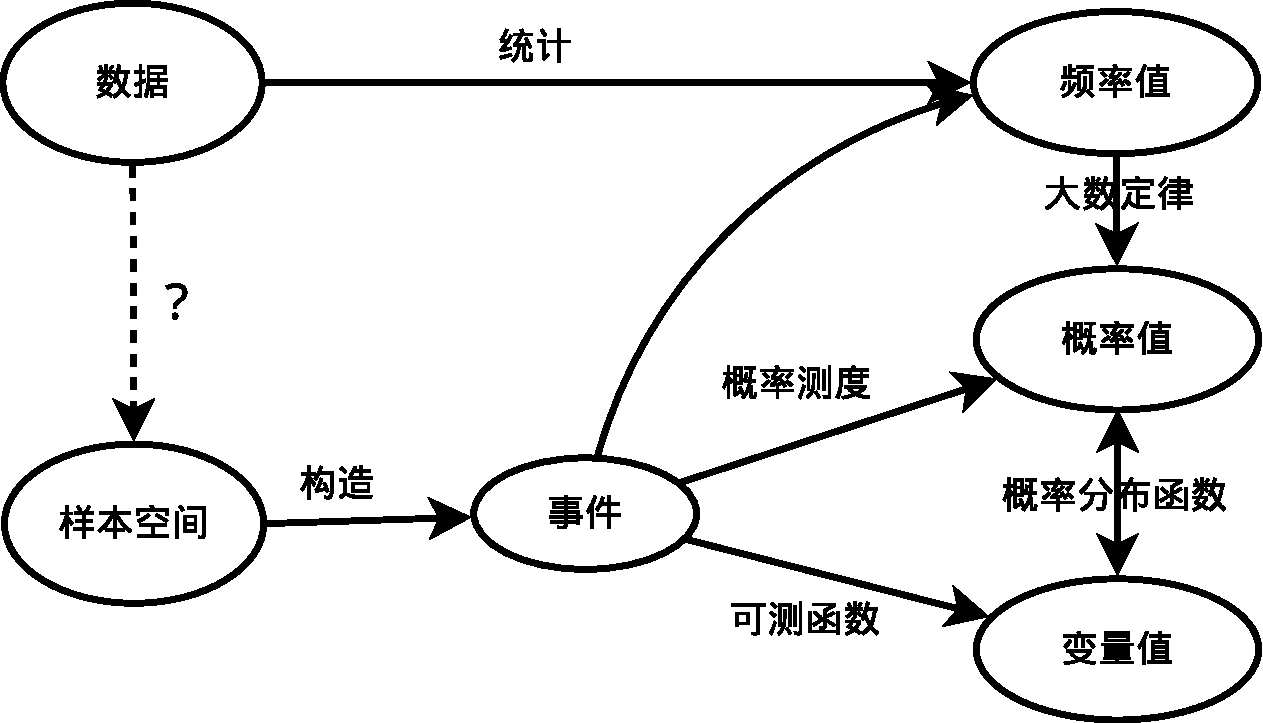
\includegraphics[width=0.6\textwidth]{probability}
%%	\caption{利用统计与概率知识解决样本空间相关问题示意图}
	\end{center}
}
      \end{block}

      %%%%%%%%%%%%%%%%%%%%%%%%%%%%%%%%%%%%%%%%%%%%%%%%%%%%%%%%%%%%%%%%%%%%%%%%%%%%%%%%%%%%%%%%%%%%%%%%%%%%%%%%%%%%
      
      \begin{block}{假定}
%        \begin{columns}[T]
%          \begin{column}{.49\linewidth}
            \begin{itemize}
            \item 过程模型只包含有限个任务 
            \item 轨迹独立地随机产生 
            \item 轨迹的产生概率是固定的
			\item 噪声假定
              \begin{itemize}
              \item 没有噪声,或
              \item 噪声导致正常轨迹以固定条件概率变为另一条任务串
              \end{itemize}
           \end{itemize}
 %         \end{column}
 %         \begin{column}{.49\linewidth}
 %           \begin{itemize}
 %           \item \alert{goal:} find the model which best expresses the observation sequence
%            \end{itemize}
%            \vskip2ex
            %\includegraphics[width=\linewidth]{dreuw/xfigures/BayesArchitectureSignLanguage_Dreuw_01Jun06}
%          \end{column}
%        \end{columns}
      \end{block}

      %%%%%%%%%%%%%%%%%%%%%%%%%%%%%%%%%%%%%%%%%%%%%%%%%%%%%%%%%%%%%%%%%%%%%%%%%%%%%%%%%%%%%%%%%%%%%%%%%%%%%%%%%%%%
      \begin{block}{完备性评价框架}
%        \begin{columns}[t]
%          \begin{column}{.75\linewidth}
            \noindent{\hskip1cm\textbf{信息单元}}
            \begin{itemize}
            \item 因需而异
              \begin{itemize}
              \item 全局完备:轨迹
              \item 局部完备:直接后继关系
              \end{itemize}
            \end{itemize}

            \vskip1ex            
            \noindent{\hskip1cm\textbf{度量指标}}
            \begin{itemize}
            \item 已知单元占比(OUR): $OUR=(no. of observed units)/(no. of
				all units)$
            \item 概率覆盖度(CV): $CV=(prob. of observed units)/(prob. of
				all units)$
            \item 完备日志长度(N): 如果日志要求完备,还有多少轨迹?
            \end{itemize}

            \vskip1ex            
            \noindent{\hskip1cm\textbf{框架结构}}
%            \begin{itemize}
					\begin{center}
            		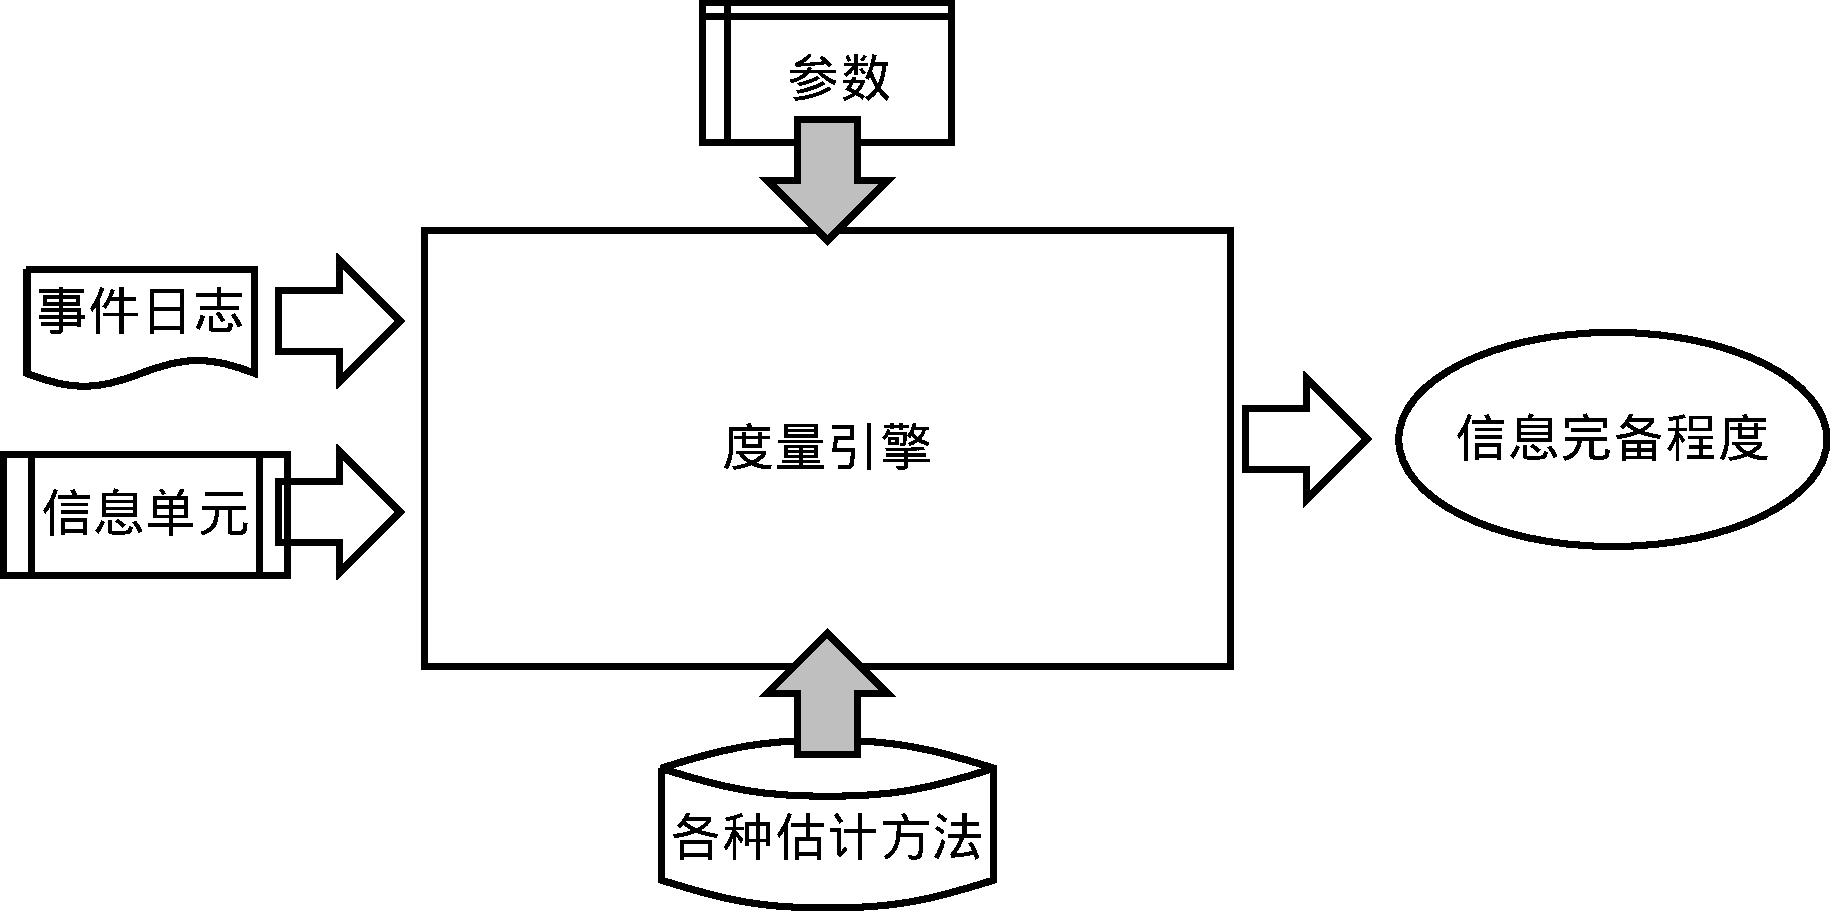
\includegraphics[width=0.7\linewidth]{figures/framework}\\[1ex]
					\end{center}
%            \end{itemize}
%          \end{column}

%          \begin{column}{.25\linewidth}
            \vskip0ex
            %%%%%%%%%%%%%%%%%%%%%%%%%%%%%%%%%%%
            \centering    
            %\includegraphics[width=0.7\linewidth]{images/figures/Boston104-1_Dreuw_01Jun06}\\[1ex]
            %\includegraphics[width=0.7\linewidth]{images/figures/Boston104-2_Dreuw_01Jun06}\\[1ex]
            %\includegraphics[width=0.7\linewidth]{images/figures/Boston104-3_Dreuw_01Jun06}\\[1ex]          
            %\includegraphics[width=0.7\linewidth]{images/u-signlanguage-BOSTON104-png-png-segments-190_fn000060-0}\\[1ex]          
%          \end{column}
%        \end{columns}

      \end{block}

      %%%%%%%%%%%%%%%%%%%%%%%%%%%%%%%%%%%%%%%%%%%%%%%%%%%%%%%%%%%%%%%%%%%%%%%%%%%%%%%%%%%%%%%%%%%%%%%%%%%%%%%%%%%%

    \end{column}
    \begin{column}{.3\linewidth}
      \begin{block}{全局完备性度量}
        \vfill
        \noindent{\textbf{形式化问题}}\\
%		\noindent{\begin{problem}[日志全局完备性问题(Global Completeness problem)]\label{prob:global}
			给定一个由未知业务过程模型$P$产生的事件日志$L$和一个置信水平$K$ ($0<K<1$),
			\begin{enumerate}
				\item 如果我们能够以置信度$K$断言日志已经全局完备,则日志长度$N$最少是多少?
				\item 我们能够以置信度$K$断言日志中出现的轨迹种类数目跟模型$P$的所有可能轨迹种类数目的比值是多少?
			\end{enumerate}
%		\end{problem}}

        \vskip1ex
        \noindent{\textbf{轨迹的概率与频率}}
	\begin{center}
	\label{tbl:tracefreqprob} 
	\begin{tabular}{lcccccccc} 
		\hline\noalign{\smallskip} 
		轨迹&$T_1$ & $T_2$& $\cdots$ & $T_{M-1}$ & $T_M$ & $T_{M+1}$ & $\cdots$ & $T_W$\\ 
		\noalign{\smallskip} \hline \noalign{\smallskip}
		概率&$p_1$ & $p_2$& $\cdots$ & $p_{M-1}$ & $p_M$ & $p_{M+1}$ & $\cdots$ & $p_W$\\ 
		\noalign{\smallskip} \hline \noalign{\smallskip}
		频率&$\frac{\mu_1}{N}$&$\frac{\mu_2}{N}$&$\cdots$&$\frac{\mu_{M-1}}{N}$&$\frac{\mu_M}{N}$&0&$\cdots$&0\\
		\hline 
	\end{tabular} 
	\end{center} 

        \vskip1ex
        \noindent{\textbf{问题解答}}
		\begin{itemize}
			\item %\begin{solution}
给定由未知模型$P$生成的日志$L$、置信水平$K$($0<K<1$)及任意正数$\varepsilon$ ($0<\varepsilon<1$), 
若要以置信度$K$断言观测到的轨迹的经验分布与真实分布的误差不超过$\varepsilon$,则日志的长度$N$最小不低于
$\frac{M^3}{4(1-K)\varepsilon^2}$\ \ \ 。
%\end{solution}
			\item %\begin{solution}
给定一个由未知模型$P$生成、包含$M$种不同轨迹且长度为$N$的事件日志$L$,及一个置信水平$K(1>k>0)$,
已知轨迹种类数目跟全部轨迹种类数目的比值,利用轨迹出现概率来估计,以置信水平$K$断言它的一个上界是
$ 1-\frac{M^\frac{3}{2}}{2\sqrt{N\left(1-K\right)}}$\ \ \ \ 。
%\end{solution}
		\end{itemize}
        \vskip1ex
        \noindent{\textbf{结论反直觉的解释}}\\
		\alert{利用已知轨迹的不断重复,来增加我们认为将要见到未知轨迹的可能性很小的信心。所以日志中不同轨迹数目越多,重复性越小,遇到未知轨迹的概率增加,日志完备性降低。}

%        \vskip1ex
%        \begin{columns}[t]
%          \begin{column}{.5\linewidth}
%            \noindent{\hskip1cm\textbf{Features}}\par
%            \begin{itemize}
%            \item \alert{appearance-based image features}: for baseline system
%              \begin{itemize}
%              \item thumb\-nails of video se\-quen\-ce fra\-mes (intensity images scaled to 32x32 pixels)
%              \item give a global description of all (manual and non-manual) features proposed in linguistic research
%              \end{itemize}
%            \item \alert{manual features}: 
%              \begin{itemize}
%              \item dominant hand \alert{tracking}: hand position,
%                hand velocity, and hand trajectory features
%              \end{itemize}
%            \end{itemize}
%          \end{column}
%          \begin{column}{.5\linewidth}
%            \vskip0ex
%            %%%%%%%%%%%%%%%%%%%%%%%%%%%%%%%%%%%%%%%%%%%%%%%%%%%%%%%
%            \centering
%            %\includegraphics[height=0.33\linewidth]{images/u-signlanguage-BOSTON104-videoBank-camera0-001_0_fn000054-0}
%            \quad\quad
%            %\includegraphics[height=0.33\linewidth]{images/u-signlanguage-BOSTON104-videoBank-camera0-090_0_fn000056-0}
%            \vskip3ex
%            %\includegraphics[height=0.4\linewidth]{images/graphs/trajectory_45_54}
%            \quad
%            %\includegraphics[height=0.4\linewidth]{images/graphs/trajectory_25_34}
%            %%%%%%%%%%%%%%%%%%%%%%%%%%%%%%%%%%%%%%%%%%%%%%%%%%%%%%%
%          \end{column}
%        \end{columns}
      \end{block}

      \begin{block}{局部完备性度量}
        \vfill
        \noindent{\textbf{形式化问题}}\\
%		\noindent{\begin{problem}[日志全局完备性问题(Global Completeness problem)]\label{prob:global}
			给定一个由未知业务过程模型$P$产生的事件日志$L$和一个置信水平$K$ ($0<K<1$),
			\begin{enumerate}
				\item 如果我们能够以置信度$K$断言日志已经局部完备,则日志长度$N$最少是多少?
				\item 我们能够以置信度$K$断言已观测到的直接后继关系种类的出现概率之和占全部直接后继出现概率的占比是多少?
			\end{enumerate}
%		\end{problem}}
        \vskip1ex
        \noindent{\textbf{DS关系的特征}}
\begin{itemize}
	\item DS关系的出现是不独立的,致全局完备方法不能直接用。
	\item 可以证明,若忽略DS出现的次数,则DS的出现概率是个常数。
\end{itemize}

        \vskip1ex
        \noindent{\textbf{轨迹的概率与频率}}\\
	\begin{center}
\begin{tabular}{lcccccc}
\hline\noalign{\smallskip}
DS关系 &$T_1$ &  $\cdots$ & $T_W$& 出现概率 &出现频率\\
\noalign{\smallskip} \hline \noalign{\smallskip}
$R_{1,1}$&$Sign(T_1,R_{1,1})$&$\cdots$&$Sign(T_W,R_{1,1})$&$p_{1,1}$&$\frac{\nu_{1,1}}{N}$\\
\noalign{\smallskip} \hline \noalign{\smallskip}
$R_{1,2}$&$Sign(T_1,R_{1,2})$&$\cdots$&$Sign(T_W,R_{1,2})$&$p_{1,2}$&$\frac{\nu_{1,2}}{N}$\\
\noalign{\smallskip} \hline \noalign{\smallskip}
$\vdots$&$\vdots$&$\cdots$&$\vdots$&$\vdots$&$\vdots$\\
\noalign{\smallskip} \hline \noalign{\smallskip}
$R_{R,R}$&$Sign(T_1,R_{R,R})$&$\cdots$&$Sign(T_W,R_{R,R})$&$p_{R,R}$&$\frac{\nu_{R,R}}{N}$\\
\hline
\end{tabular}
	\end{center} 

        \vskip1ex
        \noindent{\textbf{问题解答}}
		\begin{itemize}
			\item 如果要以置信水平$K$断定日志是局部信息完备的,则日志长度$N$至少是
$\frac{1}{\varepsilon\sqrt{1-K}}-1$, 其中$\varepsilon$是可接受的误差.
			\item 以置信水平$K$断言借助DS关系的出现概率估计出来的
已观测到的DS数量占全部DS数量的比值上界是 
$ 1-\frac{1}{(N+1)\sqrt{1-K}}$.
		\end{itemize}
%        \begin{columns}[T]
%          \begin{column}{.35\linewidth}
%            \noindent{\hskip1cm\textbf{Feature Selection}}\par
%            \begin{itemize}
%            \item \alert{concatenation} of appearance-based and manual features
%            \item \alert{sliding window} for context modeling
%            \item \alert{dimensionality reduction} by PCA and/or LDA
%            \end{itemize}
%          \end{column}
%          \begin{column}{.65\linewidth}
%            \raggedleft
%            %\includegraphics[width=.95\linewidth]{images/xfigures/CompositeFeature_Dreuw_28Sep06}%
%          \end{column}
%        \end{columns}
%
%        \vskip5ex
%        \begin{columns}[T]
%          \begin{column}{.35\linewidth}
%            \noindent{\hskip1cm\textbf{Model Combination}}\par
%            \begin{itemize}
%            \item \alert{log-linear combination} of independently
%              trained models
%            \item profit from independent alignments (\eg performing well for long and short words)
%            \item profit from different feature extraction approaches
%            \end{itemize}
%          \end{column}
%          \begin{column}{.65\linewidth}
%            \raggedleft
%            %\includegraphics[width=\linewidth]{images/xfigures/CompositeModels_Dreuw_17Apr07}
%          \end{column}
%        \end{columns}
%
%
%        %%%%%%%%%%%%%%%%%%%%%%%%%%%%%%%%%%%%%%%%%%%%%%%%%%%%%%%
      \end{block}

    \end{column}

    %%%%%%%%%%%%%%%%%%%%%%%%%%%%%%%
    
    \begin{column}{.3\linewidth}

      \begin{block}{日志噪声处理}
        %%%%%%%%%%%%%%%%%%%%%%%%%%%%%%%%%%%%%%%%%%%%%%%%%%%%%%%
        \vskip1ex
        \noindent{\textbf{概念辨析}}
		\begin{center}
		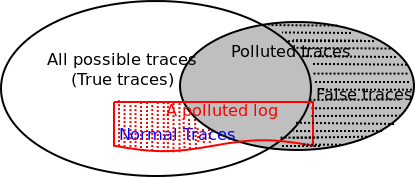
\includegraphics[width=0.6\textwidth]{figures/traces}
		\end{center}
		
        \vskip1ex
        \noindent{\textbf{问题形式化}}
		\begin{itemize}
	\item \alert{非真轨迹识别问题(False trace identification problem)}给定一个由未知过程模型产生的污损日志$L$,以及一个污染矩阵$\mathbf{M}$,日志中的
哪些轨迹最有可能是非真轨迹?
\item \alert{非真轨迹发现问题(False trace discovery problem)}给定一个由未知过程模型产生的污损日志$L$,日志中的哪些轨迹最有可能是非真轨迹?
		\end{itemize}

        \vskip1ex
        \noindent{\textbf{轨迹的产生概率与出现概率}}
		\begin{center}
		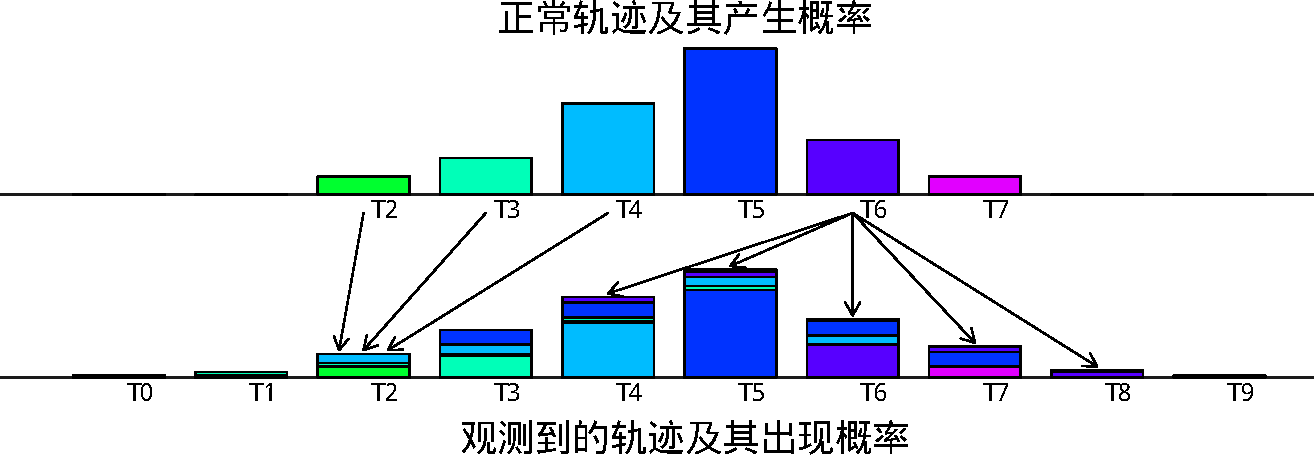
\includegraphics[width=0.6\textwidth]{figures/pollution}
		\end{center}

        \vskip1ex
        \noindent{\textbf{轨迹的产生概率、污染矩阵与出现概率的关系}}
\begin{tabular}{cccccccc|c|c}
\hline\noalign{\smallskip}
Trace&~~$T_1$~~&~~$T_2$~~& $\cdots$&~~$T_M$&~~$T_{M+1}$&$\cdots$&~~$T_W$&prob.unobserv&Gen. prob.\\
\noalign{\smallskip} \hline \noalign{\smallskip}
$T_1$&$p_{1,1}$&$p_{1,2}$&$\cdots$&$p_{1,M}$&$p_{1,M+1}$&$\cdots$&$p_{1,W}$&$u_1$&\colorbox{Gray}{$g_1$}\\
$T_2$&$p_{2,1}$&$p_{2,2}$&$\cdots$&$p_{2,M}$&$p_{2,M+1}$&$\cdots$&$p_{2,W}$&$u_2$&\colorbox{Gray}{$g_2$}\\
$\vdots$&$\vdots$&$\vdots$&$\cdots$&$\vdots$&$\vdots$&$\cdots$&$\vdots$&$\vdots$&\colorbox{Gray}{$\vdots$}\\
$T_M$&$p_{M,1}$&$p_{M,2}$&$\cdots$&$p_{M,M}$&$p_{M,M+1}$&$\cdots$&$p_{M,W}$&$u_M$&\colorbox{Gray}{$g_M$}\\
\noalign{\smallskip} \hline \noalign{\smallskip}
Occur. prob.&\colorbox{Gray}{$p_1$}&\colorbox{Gray}{$p_2$}&\colorbox{Gray}{$\cdots$}&\colorbox{Gray}{$p_M$}&\colorbox{Gray}{$p_{M+1}$}&\colorbox{Gray}{$\cdots$}&\colorbox{Gray}{$p_W$}&\colorbox{Gray}{$p_U$}\\
\noalign{\smallskip} \hline \noalign{\smallskip}
Occur. freq. & $f_1$ & $f_2$ & $\cdots$ & $f_M$ & $f_{M+1}$ & $\cdots$ & $f_W$ & $0$\\
\noalign{\smallskip} \hline \noalign{\smallskip}
Occur. times&$n_1$&$n_2$&$\cdots$&$n_M$&$n_{M+1}$&$\cdots$&$n_W$&$0$\\
\hline
\end{tabular}
        \vskip1ex
        \noindent{\textbf{问题解决}}
		\begin{itemize}
			\item 非真轨迹识别
			\begin{enumerate}
		\item 统计轨迹出现频率
		\item 最小化出现频率与概率之间的误差函数来估计潜在生成概率,
$	\argmin_{\mathbf{G}}Q^2=\argmin_{\mathbf{G}} p^2_U
N^2+\sum_{i=1}^M(f_i-p_i)^2 \frac{N}{f_i}$
其中约束条件是$\sum_{i=1}^Mg_i=1$, $g_i\geq 0$.
		\item 进行$\chi^2$检验,识别非真轨迹(概率为(或非常接近)0者).
	\end{enumerate}
\item 非真轨迹发现:交互迭代
		\end{itemize}
        %\includegraphics[width=0.33\linewidth]{images/pca-ldaw/ldaw}%
        %\includegraphics[width=0.33\linewidth]{images/pca-pcaw/pcaw}%
        %\includegraphics[width=0.33\linewidth]{images/language-model/lm-scale}%
        %%%%%%%%%%%%%%%%%%%%%%%%%%%%%%%%%%%%%%%%%%%%%%%%%%%%%%%

      \end{block}
      
%      \vskip-2ex
%      \begin{columns}[t]
%        ~~
%        \begin{column}{.57\linewidth}
%          \begin{block}{Example Results}   
%            \noindent{\hskip1cm\textbf{Correct Examples}}        
%            \hrule
%            \begin{tabular}{@{}>{\small}c@{}>{\small}c@{}>{\small}c@{}>{\small}c}
%              IX-1P & \ \ FIND & \ \ SOMETHING-ONE & \ \ BOOK\\
%              \textcolor{black}{IX-1P} & \ \ \textcolor{black}{FIND} & \ \ \textcolor{black}{SOMETHING-ONE} & \ \ \textcolor{black}{BOOK}
%            \end{tabular}
%            \hrule
%            \begin{tabular}{@{}>{\small}c@{}>{\small}c@{}>{\small}c@{}>{\small}c@{}>{\small}c@{}>{\small}c@{}>{\small}c@{}>{\small}c}
%              JOHN & \ \ FISH & \ \ WONT & \ \ EAT & \ \ BUT & \ \ CAN & \ \ EAT & \ \ CHICKEN\\
%              \textcolor{black}{JOHN} & \ \ \textcolor{black}{FISH} & \ \ \textcolor{black}{WONT} & \ \ \textcolor{black}{EAT} & \ \ \textcolor{black}{BUT} & \ \ \textcolor{black}{CAN} & \ \ \textcolor{black}{EAT} & \ \ \textcolor{black}{CHICKEN}
%            \end{tabular}
%            \hrule
%            \begin{tabular}{@{}>{\small}c@{}>{\small}c@{}>{\small}c}
%              LOVE & \ \ JOHN & \ \ WHO\\
%              \textcolor{black}{LOVE} & \ \ \textcolor{black}{JOHN} & \ \ \textcolor{black}{WHO}
%            \end{tabular}
%            \hrule
%            \begin{tabular}{@{}>{\small}c@{}>{\small}c@{}>{\small}c@{}>{\small}c@{}>{\small}c}
%              JOHN & \ \ BUY & \ \ YESTERDAY & \ \ WHAT & \ \ BOOK\\
%              \textcolor{black}{JOHN} & \ \ \textcolor{black}{BUY} & \ \ \textcolor{black}{YESTERDAY} & \ \ \textcolor{black}{WHAT} & \ \ \textcolor{black}{BOOK}
%            \end{tabular}
%            \hrule          
%            \vskip2ex
%            \noindent{\hskip1cm\textbf{Incorrect Examples}}\par                              
%            \hrule
%            \begin{tabular}{@{}>{\small}c@{}>{\small}c@{}>{\small}c@{}>{\small}c@{}>{\small}c@{}>{\small}c}
%              MARY & \ \ VEGETABLE & \ \ KNOW & \ \ IX & \ \ LIKE & \ \ CORN\\
%              \textcolor{black}{MARY} & \ \ \textcolor{black}{VEGETABLE} & \ \ \textcolor{black}{KNOW} & \ \ \textcolor{black}{IX} & \ \ \textcolor{black}{LIKE} & \ \ \textcolor{red}{MARY}
%            \end{tabular}
%            \hrule
%            \begin{tabular}{@{}>{\small}c@{}>{\small}c@{}>{\small}c@{}>{\small}c@{}>{\small}c@{}>{\small}c@{}>{\small}c}
%              JOHN & \ \ IX & \ \ GIVE & \ \ MAN & \ \ IX & \ \ NEW & \ \ COAT\\
%              \textcolor{black}{JOHN} & \ \ \textcolor{black}{IX} & \ \ \textcolor{red}{WOMAN} & \ \ \textcolor{black}{\underline{\phantom{MAN}}} & \ \ \textcolor{black}{\underline{\phantom{IX}}} & \ \ \textcolor{black}{NEW} & \ \ \textcolor{black}{COAT}
%            \end{tabular}
%            \hrule
%            \begin{tabular}{@{}>{\small}c@{}>{\small}c@{}>{\small}c@{}>{\small}c}
%              & \ \ LIKE & \ \ CHOCOLATE & \ \ WHO\\
%              \textcolor{green}{JOHN} & \ \ \textcolor{black}{LIKE} & \ \ \textcolor{black}{CHOCOLATE} & \ \ \textcolor{black}{WHO}
%            \end{tabular}
%            \hrule
%            \begin{tabular}{@{}>{\small}c@{}>{\small}c@{}>{\small}c@{}>{\small}c@{}>{\small}c}
%              JOHN & \ \ [UNKNOWN] & \ \  & \ \ BUY & \ \ HOUSE\\
%              \textcolor{black}{JOHN} & \ \ \textcolor{red}{FUTURE} & \ \ \textcolor{green}{NOT} & \ \ \textcolor{black}{BUY} & \ \ \textcolor{black}{HOUSE}
%            \end{tabular}
%            \hrule
%            \vspace{-1ex}            
%          \end{block}
%        \end{column}
%        ~
%        \begin{column}{.4\linewidth}
%          \begin{block}{RWTH-BOSTON-104 Database}   
%            %%%%%%%%%%%%%%%%%%%%%%%%%%%%%%%%%%%%%%%%%%%%%%%%%%%%%%
%            \noindent{\hskip1cm\textbf{Corpus Statistics}}        
%            \begin{table}
%              \centering
%              %\footnotesize
%              %\caption{Corpus Statistics}
%              \begin{tabular}{@{} p{.5\linewidth}  r r @{}}
%                \toprule
%                                 & Training   &  Test \\
%                \midrule
%                sentences        & 161        &  40   \\
%                running words    & 710        & 178   \\
%                frames           & 12422      & 3324  \\
%                vocabulary       & 103        &  65   \\
%                singletons       &  27        &   9   \\
%                OOV              & -          &   1   \\
%                \bottomrule
%              \end{tabular}
%            \end{table}
%            \vskip2ex
%            %%%%%%%%%%%%%%%%%%%%%%%%%%%%%%%%%%%%%%%%%%%%%%%%%%%%%%
%            \noindent{\hskip1cm\textbf{LM Perplexities}}        
%            \begin{table}
%              \centering
%              %\caption{}
%              \begin{tabular}{@{} p{.8\linewidth} r @{}}
%                \toprule
%                LM type     & $PP$ \\
%                \hline
%                zerogram    & 106.0 \\
%                unigram     & 36.8 \\
%                bigram      & 6.7 \\
%                trigram     & 4.7 \\
%                \bottomrule
%              \end{tabular}
%            \end{table}
%            %%%%%%%%%%%%%%%%%%%%%%%%%%%%%%%%%%%%%%%%%%%%%%%%%%%%%%%
%            \vskip2ex
%            Database is publicly available
%          \end{block}
%        \end{column}
%      \end{columns}
                
      \begin{block}{总结与展望}
	\begin{itemize}
		\item 总结及本文的创新之处
			\begin{itemize}
				\item 辨析完备性与噪声的相关观念,形式化相关问题
				\item 提出日志全局完备性的度量方法
				\item 提出日志局部完备性的度量方法
				\item 提出日志中非真轨迹的FATILP方法
				\item 日志完备性的方法提供ProM插件的开源实现
			\end{itemize}
		\item 展望
			\begin{itemize}
				\item 充分利用日志特征与噪声模型,研究新的方法
				\item 研究将噪声问题与完备性问题一起解决的方法。
%				\item 提出统一的完备性评估框架
			\end{itemize}
	\end{itemize}
        \vspace{-1ex}
      \end{block}
%%%%%%%%%%%%%%%%%%%%%%%%%%%%%%%%%%%%%%%%%%%%%%%%%%%%%%%

    \end{column}
  \end{columns}
\end{frame}

\end{document}


%%%%%%%%%%%%%%%%%%%%%%%%%%%%%%%%%%%%%%%%%%%%%%%%%%%%%%%%%%%%%%%%%%%%%%%%%%%%%%%%%%%%%%%%%%%%%%%%%%%%
%%% Local Variables: 
%%% mode: latex
%%% TeX-PDF-mode: t
%%% End: 
